\subsection{Instruction Decoding}
\label{group__instructiondecoder}\index{Instruction Decoding@{Instruction Decoding}}
An InstructionDecoder interprets a sequence of bytes according to a given machine language and transforms them into an instruction representation. It determines the opcode of the machine instruction, translates that opcode to an Operation object, uses that Operation to determine how to decode the instruction's Operands, and produces a decoded Instruction.


\begin{DoxyImage}
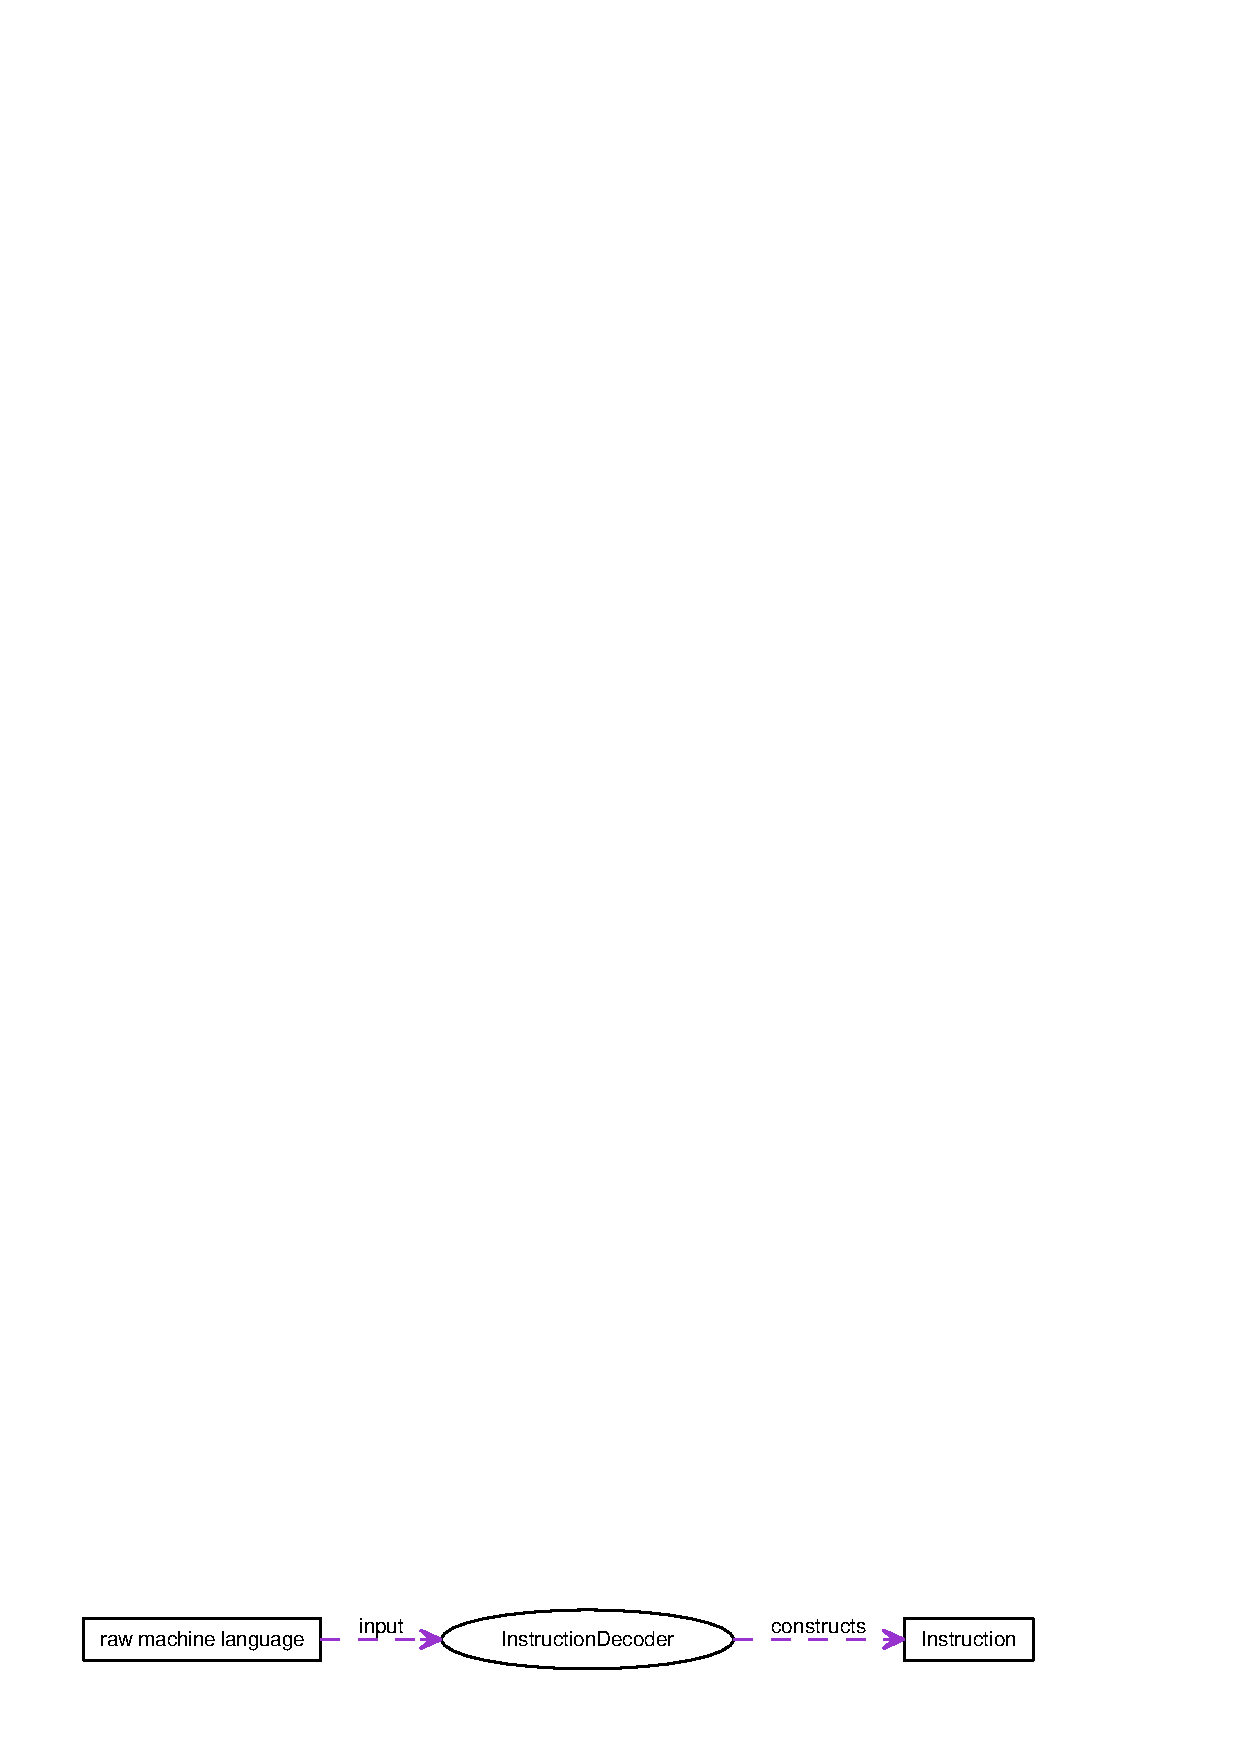
\includegraphics{decoder_use}
\caption{The InstructionDecoder's inputs and outputs}
\end{DoxyImage}
 Instruction decoders are built from the following elements:
\begin{DoxyItemize}
\item A function to find and extract an opcode given a pointer into a buffer that points to the beginning of a machine instruction
\item A table that, for a particular architecture, maps opcodes to Operations and functions that decode Operands
\end{DoxyItemize}

From these elements, it is possible to generalize the construction of Instructions from Operations and Operands to an entirely platform-\/independent algorithm. Likewise, much of the construction of the ASTs representing each operand can be performed in a platform-\/independent manner. 